\chapter{Implementierung}
\label{chapter:Implementierung}

\section{Auswahl der Bauteile}
\label{section:Auswahl_der_Bauteile}

Für das Projekt wurden die echtzeitfähige Steuerung, die Batterie, der Motor und die zugehörige Steuerung vorgegeben. Alle weiteren Bauteile mussten bestellt werden.

\section{Schaltplan}
\label{section:Schaltplan}


\myboxy{
	\begin{itemize}
		\item Funktion (=Anlage) und Ortskennzeichen (+Ort) definieren. Funktionales Engineering.
		\item Bauteilkennzeichnung (BMK) festlegen.
		\item Aderfarben und Querschnitt definieren.
		\item Ausgewählte Bauteile in die Schaltung integrieren.
		\item Nicht vorhandene Bauteile selbst erstellen.
		      \begin{itemize}
			      \item Bauteile sortiert hinzufügen: Spannungsversorgung, Steuerung (Eingang, dann Ausgang), Lastkreis und Sonderfunktionen.
		      \end{itemize}
	\end{itemize}}{To-do}{\textwidth}



Zu Beginn der Erstellung des Schaltplans sollten die Funktions- und Ortskennzeichen sowie die Beschriftung der Bauteile und Leitungen festgelegt werden. Bei der Verdrahtung ist es erforderlich, die Aderfarben den entsprechenden Spannungspotenzialen zuzuordnen.

\subsection{Betriebsmittelbezeichnung}
\label{Schaltplan:BMK}

Ein Betriebsmittel besteht aus verschiedenen Kennzeichen: dem Funktionskennzeichen (=), dem Ortskennzeichen (+) und dem Betriebsmittelkennzeichen (-). Früher wurde das Funktionskennzeichen als „Anlage“ bezeichnet. In der neuen DIN EN IEC 81346-2 \cite{DIN_EN_IEC_81346-2} wurde diese Bezeichnung jedoch auf „Funktion“ geändert.

\subsubsection{Funktionskennzeichen}
Das Funktionskennzeichen beschreibt eine bestimmte Funktion im Schaltplan, wie beispielsweise die Spannungsversorgung oder die Steuerung (siehe Tabelle \ref{BMK:tab:funktionskennzeichen}).

\pagebreak[1]
\begin{table}[!ht]
	\centering
	\caption{Schaltplan – Funktionskennzeichen (=)}
	\label{BMK:tab:funktionskennzeichen}
	\begin{tabular}{ll}
		\hline
		\textbf{Abkürzung}      & \textbf{Bezeichnung} \\ \hline
		\multicolumn{1}{l|}{SV} & Spannungsversorung   \\
		\multicolumn{1}{l|}{ES} & Eingänge Steuerung   \\
		\multicolumn{1}{l|}{AS} & Ausgänge Steuerung   \\
		\multicolumn{1}{l|}{KO} & Kommunikation        \\
		\multicolumn{1}{l|}{AT} & Antrieb              \\
		\multicolumn{1}{l|}{NA} & Not-Aus              \\ \hline
	\end{tabular}
\end{table}
\pagebreak[1]

\subsubsection{Ortskennzeichen}
Das Ortskennzeichen gibt an, an welchem Ort ein Bauteil installiert ist. Beispielsweise gibt es im Fahrzeug eine Steuereinheit und eine Batterieeinheit. Im Schaltplan wird dadurch deutlich, welche Verbindungen zwischen verschiedenen Orten bestehen. Das Ortskennzeichen erleichtert zudem die Wartung und Installation des Systems.

\pagebreak[1]
\begin{table}[!ht]
	\centering
	\caption{Schaltplan – Ortskennzeichen (+)}
	\label{bmk:tab:ortskennzeichen}
	\begin{tabular}{ll}
		\hline
		\textbf{Abkürzung}       & \textbf{Bezeichnung} \\ \hline
		\multicolumn{1}{l|}{POD} & Fahrzeug             \\
		\multicolumn{1}{l|}{BE}  & Batterieeinheit      \\
		\multicolumn{1}{l|}{SE}  & Steuereinheit        \\
		\multicolumn{1}{l|}{AE}  & Antriebseinheit      \\ \hline
	\end{tabular}
\end{table}
\pagebreak[1]

\subsubsection{Betriebsmittelkennzeichen}
Das Betriebsmittelkennzeichen bezeichnet das spezifische Bauteil. Die genaue Zuordnung der Bezeichnungen ist in der DIN EN IEC 81346-2 geregelt. Die für das Projekt relevanten Betriebsmittelkennzeichen sind in Tabelle \ref{bmk:tab:betriebsmittelkennzeichen} aufgeführt.



\pagebreak[1]
\begin{table}[!ht]
	\centering
	\caption{Schaltplan – Betriebsmittelkennzeichen (-) \cite{DIN_EN_IEC_81346-2}}
	\label{bmk:tab:betriebsmittelkennzeichen}
	\begin{tabular}{|l|lll|}
		\hline
		\textbf{Abkürzung}       & \textbf{Klassenname}                            & \multicolumn{1}{l|}{\textbf{Allgemeine Bedeutung}} \\ \hline
		\multicolumn{1}{|l|}{FC} & \makecell[l]{Überstromschutzobjekt}             & \multicolumn{1}{l|}{Sicherung}                     \\ \hline
		\multicolumn{1}{|l|}{GB} & \makecell[l]{Erzeugungsobjekt für elektrische                                                        \\Energie durch chemische Energie} & \multicolumn{1}{l|}{Batterie} \\ \hline
		\multicolumn{1}{|l|}{KE} & \makecell[l]{Elektrische Signale                                                                     \\verarbeitendes Objekt}   & \multicolumn{1}{l|}{Steuerung} \\ \hline
		\multicolumn{1}{|l|}{MA} & \makecell[l]{Elektromagnetisches                                                                     \\Rotationsantriebsobjekt} & \multicolumn{1}{l|}{Motor} \\ \hline
		\multicolumn{1}{|l|}{QA} & \makecell[l]{Stromsteuerungsobjekt}             & \multicolumn{1}{l|}{Relais}                        \\ \hline
		\multicolumn{1}{|l|}{RL} & \makecell[l]{Bewegungsbegrenzungsobjekt}        & \multicolumn{1}{l|}{Bremse}                        \\ \hline
		\multicolumn{1}{|l|}{SF} & \makecell[l]{Gesichtsinteraktionsobjekt}        & \multicolumn{1}{l|}{Schalter}                      \\ \hline
		\multicolumn{1}{|l|}{TB} & \makecell[l]{Stromkonvertierungsobjekt}         & \multicolumn{1}{l|}{Transformator}                 \\ \hline
		\multicolumn{1}{|l|}{WD} & \makecell[l]{Niederspannungsenergie Leitobjekt} & \multicolumn{1}{l|}{Leitung/Kabel}                 \\ \hline
		\multicolumn{1}{|l|}{XD} & \makecell[l]{Niederspannungs-Verbindungsobjekt} & \multicolumn{1}{l|}{Klemme, Stecker oder Buchse}   \\ \hline
	\end{tabular}
\end{table}
\pagebreak[1]

Bei einer vollständigen Betriebsmittelbezeichnung sieht das Kennzeichen des Betriebsmittels folgendermaßen aus:

\begin{center} =ES2+SE1-10QA1 \end{center}

Die Betriebsmittelbezeichnung =ES2+SE1-10QA4 besagt, dass es sich um die Eingänge der Steuerung (=ES) handelt, wobei es zwei Funktionen gibt. Der Ort ist in der Steuereinheit (+SE) verortet, und das Betriebsmittel selbst ist ein Relais, das auf der Seite 10 des Schaltplans zu finden ist.

Das Kennzeichen umfasst sowohl das Funktions- als auch das Ortskennzeichen, die jeweils mit einer fortlaufenden Nummer versehen sind. Das Betriebsmittelkennzeichen enthält zwei Nummerierungen: Die erste gibt an, auf welcher Seite des Schaltplans sich das Betriebsmittel befindet, während die zweite die fortlaufende Nummerierung des Bauteils darstellt.\\
Im Schaltplan wird das Betriebsmittel lediglich durch das Betriebsmittelkennzeichen (-) dargestellt, während das Funktions- und Ortskennzeichen im Zeichnungskopf angegeben ist.

\newpage

\subsection{Verdrahtung Konventionen}
\label{section:Verdrahtung_Konventionen}
Für die Verdrahtung müssen den Spannungspotenzialen verschiedene Farben zugewiesen werden. Diese Zuordnungen sind in Tabelle \ref{Verdrahtung_Konventionen:tab:Zuordnung} aufgeführt.
\pagebreak[1]
\begin{table}[ht!]
	\centering
	\caption{Verdrahtung Konvention – Aderfarben}
	\label{Verdrahtung_Konventionen:tab:Zuordnung}
	\begin{tabular}{llccl}
		\hline
		\textbf{Name} & \textbf{Fabe}                 & \textbf{U in V} & \textbf{A in mm$^2$} & \textbf{Funktion} \\ \hline
		              & \multicolumn{1}{l|}{Rot}      & $x$             & 1                    &                   \\
		              & \multicolumn{1}{l|}{Blau}     & $x$             & 1                    &                   \\
		              & \multicolumn{1}{l|}{Schwarz}  & $x$             & 1                    &                   \\
		              & \multicolumn{1}{l|}{Schwarz}  & $< 48$          & 50                   &                   \\
		              & \multicolumn{1}{l|}{Viollett} & $x$             & 1                    &                   \\ \hline
	\end{tabular}
\end{table}
\pagebreak[4]


\section{Simulation mit Simulink}
\label{section:Simulation}

\myboxy{
	\begin{itemize}
		\item
	\end{itemize}
}{To-do}{\textwidth}


\subsection{}





















\newpage

\section{Distanzmessung}

\myboxy{
	\begin{itemize}
		\item + Anschlüsse herauszufinden vier anschlüsse gefunden.
		\item + Was für Aufgaben haben die Anschlüsse?
		      \subitem Was für ein Kommunikationsprotokol hat der Sensor?
		      \subitem Asynchron und seriell mit Baudrate 115200. (Ozilloskop)
		\item mit einem ESP32 die Sensordaten lesen.
		\item Nachrichtdekodierung (Controller MCU)
		      \subitem Ox24 Start (Nachricht start)
		      \subitem 0x26 Stopp (Nachricht ende)
		      \subitem 24 30 30 30 33 32 36 30 30 32 39 26 (Stopp signal)
		      \subitem 24 30 30 30 33 32 36 30 31 33 30 26 (Laser an)
		      \subitem 24 30 30 30 32 32 31 32 33 26 (Messen)
	\end{itemize}}{To-do}{\textwidth}


Der Sensor von Pepperl+Fuchs wurde ursprünglich für die Distanzmessung angeschafft. Da dieser Sensor jedoch sehr teuer ist und wir nicht das Risiko eines möglichen Schadens im Vakuum eingehen wollten, wurde nach einer kostengünstigen Alternative gesucht.\\
Die Idee bestand darin, ein Entfernungsmessgerät von PARKSIDE zu verwenden und den Sensor aus dem Gerät zu entfernen. Die Messwerte werden anschließend mit einer MCU decodiert.

\subsection{Verbindung}
Der Sensor ist über ein Flachbandkabel mit der Hauptplatine verbunden, wie in Abbildung \ref{img_2_2:sen_dis_parkside:1} zu sehen ist. Auf der Hauptplatine befinden sich vier ungenutzte Lötstellen. Mithilfe eines Oszilloskops haben wir diese Lötstellen analysiert und festgestellt, dass Leitung eins eine Spannung von 3,3 V führt und Leitung vier als GND dient. Die Leitungen zwei und drei übertragen digitale Signale und fungieren als Datenleitungen.\\
Wenn zwei Leitungen für die Datenübertragung vorhanden sind, kann die Kommunikation bei einer zweiadrigen Verbindung entweder synchron oder asynchron erfolgen. Ist die Kommunikation synchron, dient eine der Leitungen als Taktleitung (Clock). Andernfalls, bei einer asynchronen Kommunikation, ist eine Leitung der Sender (TX) und die andere der Empfänger (RX). Dies ermöglicht eine Vollduplex-Übertragung.
Der Sensor komuniziert mit einem Bussystem.



\pagebreak[1]
\begin{figure}[ht]
	\begin{center}
		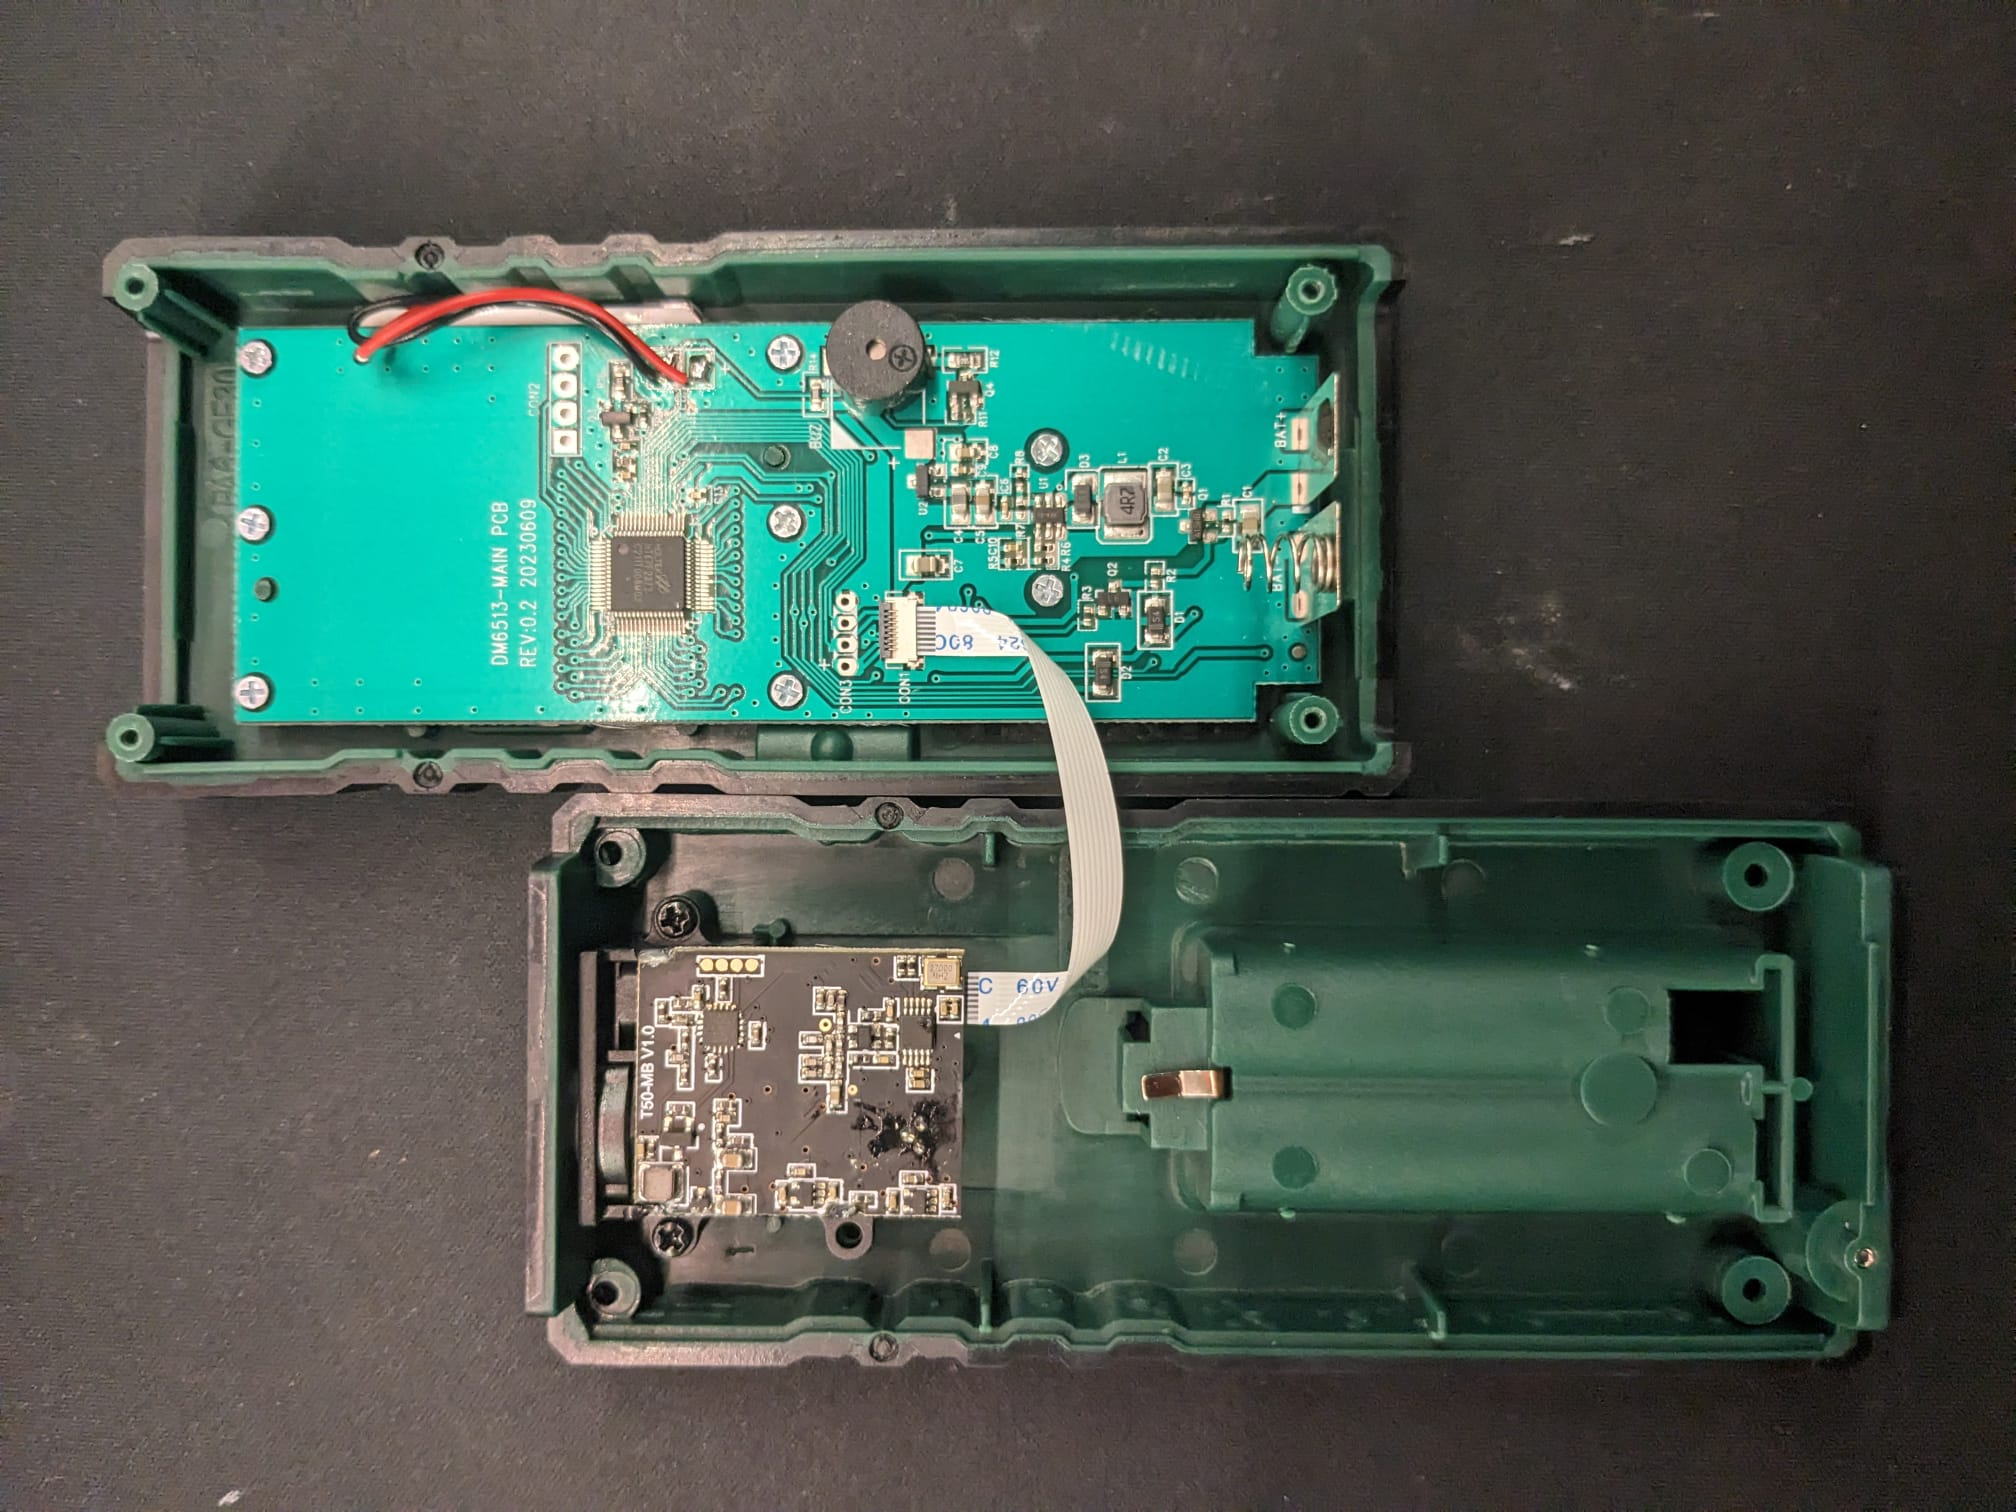
\includegraphics[width=1\textwidth]{img/2_sen/dis_parkside_1_outside.png}
		\caption{PARKSIDE – Distanzsensor – Innenaufbau}
		\label{img_2_2:sen_dis_parkside:1}
	\end{center}
\end{figure}
\pagebreak[1]

\pagebreak[1]
\begin{table}[ht]
	\centering
	\caption{PARKSIDE – Pin Mapping – Distanzsensor}
	\label{parkside:pinmapping}
	\begin{tabular}{l|ll}
		\hline
		\textbf{Pin} & \textbf{Farbe} & \textbf{Funktion} \\ \hline
		1            & Rot            & 3V3               \\
		2            & Weiß           & RX (receiver)     \\
		3            & Gelb           & TX (transmitter)  \\
		4            & Schwarz        & GND               \\ \hline
	\end{tabular}
\end{table}
\pagebreak[1]
